\section{Description of the Algorithm}

Early detection of melanoma greatly increases the chances of successful treatment. A biopsy can be performed in order to gain a definitive diagnosis. However, biopsies are invasive, painful and take time. There are also visual markers Dermatologists look for in order to make a risk assessment. The ABCD Rule, also known as Stokes or TDS Calculation, looks for 4 sets of features. Based on the features the Total Dermoscopy Score (TDS) is calculated.

The 4 sets of features are Asymmetry (A), Border Irregularity (B), Color (C) and Differential Structure or Diameter (D).

Asymmetry can have a value of 0, 1 or 2 depending on the symmetry of the lesion. Where 0 is symmetric and 2 is asymmetric. A value of 1 indicates at least one axis was found across which symmetry exists. The Border score is an integer value from 0 to 8 indicating the presence of border irregularities in 8 regions. Color is an integer value from 1 to 6 indicating the presence of one to six specific colors. Similarly, the value for D indicates the presence of one to five distinct structures or textures. Alternatively, in some literature\cite{Siddiq_2015} D is defined as Diameter, where a diameter greater than 6mm results in a value of 5, otherwise 1.

The final TDS Score is the weighted sum of the ABCD Values and is in the range 1.0 to 8.9.

\begin{equation}
\label{eq:tds_formula}
TDS = A * 1.3 + B * 0.1 + C * 0.5 + D * 0.5
\end{equation}

A diagnosis can be made based on the TDS Score according to the following table:

\begin{table}[H]
\centering
\small
    \begin{tabular}{ | l | p{3.5cm} | l | p{3.5cm} |}
    \hline
    Evaluation & TDS Score \\ \hline
    Benign & \textless  4.75  \\ \hline
    Suspicious & 4.75 to 5.45  \\ \hline
    Malignant & \textgreater  5.45  \\ \hline

    \end{tabular}

    \caption{TDS Evaluation\cite{Weigert_2012}}
    \label{fig:tds_eval}

\end{table}

\subsection{Adaptation for use in a smart phone application}

The ABCD Rule, also known as the Total \textbf{\textit{Dermoscopy}} Score, is really only applicable to images captured using a dermatoscope. Especially the differential structures are only visible on dermatoscopic images where the subsurface structures are made visible\cite{Fernandez_Alcon_2009}.

Since the D component is not applicable to images captured with a smart phone this project will use a modified TDS without the D component. The original TDS formula \ref{eq:tds_formula} can have values ranging from 1 to 8.9 and D can be 0.5 to 2.5. Without D  the TDS can have values between 0.5 and 6.4.

\begin{equation}
\label{eq:tds_modified}
TDS_{mod} = A * 1.3 + B * 0.1 + C * 0.5
\end{equation}

This results in a bening cuttoff score of 3.2 and malignagnt cuttoff of 3.7.

\begin{table}[H]
\centering
\small
    \begin{tabular}{ | l | p{3.5cm} | l | p{3.5cm} |}
    \hline
    Evaluation & Score \\ \hline
    Benign & \textless  3.20  \\ \hline
    Suspicious & 3.20 to 3.7  \\ \hline
    Malignant & \textgreater  3.7  \\ \hline

    \end{tabular}

    \caption{Adapted TDS Evaluation}
    \label{fig:tds_mod_eval}

\end{table}


\section{Automatic Calculation of ABCD Values}

The ABCD Rule is used by Dermatologists to differentiate benign from malignant melanocytic tumors. It is a clearly defined rule based on easily recognizable visual features. Clinicians with limited dermoscopy experience achieve better results using the ABCD rule than other methods \cite{Weigert_2012}. The following sections detail methods to automate the calculation of the ABCD scores.

\subsection{Asymmetry}
The "Center of mass" method of measuring asymmetry is relatively easy to calculate and is more accurate compared to other complex algorithms \cite{Premaladha_2014}.

This algorithm begins by calculating an array of radii from the lesion's center of mass to border for each of 360 degrees. The coordinates for the center of mass are calculated from the sum of all x and y coordinates of pixels within the lesion's border each divided by the sum of pixels.

For each of the 360 radii $r_i$ a score is calculated by comparing the lengths of pairs of radii that are symmetric across $r_i$. If the lengths of the pair of symmetric radii have a difference of less than 10\% then a point is given. The sum of points is the $SFA_i$ (Score For Axis) for $r_i$.

\begin{figure}[H]
    \centering
    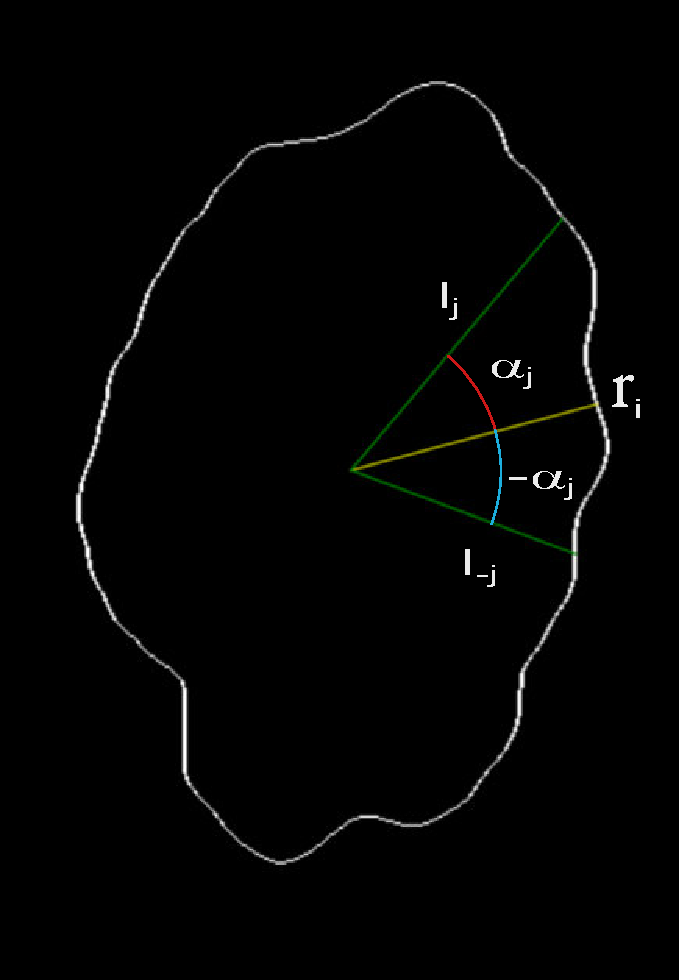
\includegraphics[height=7cm,keepaspectratio]{assets/assymertry/asymmetry_01.pdf}
    \caption{Calculate SFA for $r_i$}
    \label{fig:sfa}
\end{figure}


 The radius with the maximum SFA score is defined as the major axis of symmetry. The SFA of the major axis as well as the perpendicular are stored. The Asymmetry score is evaluated as follows:


\begin{table}[H]
\centering
\small
    \begin{tabular}{ | l | p{3.5cm} | l | p{3.5cm} |}
    \hline
    SFA Results & Description & Asymmetry Score \\ \hline
    \specialcell[t]{major axis $\geq$ 140 \\ minor axis $\geq$ 140} & Symmetric across both axis & 0  \\ \hline
    \specialcell[t]{major axis $\geq$ 140 \\ minor axis $\textless$ 140} & Symmetric across one axis & 1  \\ \hline
    \specialcell[t]{major axis \textless 140 \\ minor axis \textless 140} & Asymmetric & 2  \\ \hline


    \end{tabular}

    \caption{TDS Evaluation\cite{Weigert_2012}}
    \label{fig:tds_eval}

\end{table}

\subsection{Border}
An image is generated where only the pixels at the border or the lesion are visible, the rest of the image is black. The pixels are gathered sequentially into an array starting at any arbitrary border pixel and traversing the border continually. It's important that the sequential order of the pixels be maintained since the change in angle and distance to the lesions center will be measured.

\begin{figure}[H]
    \centering
    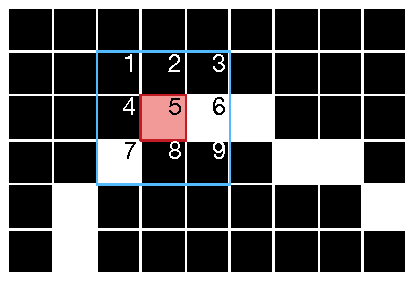
\includegraphics[height=6cm,keepaspectratio]{assets/border/travers_grid.pdf}
    \caption{Traverse the border sequentially}
    \label{fig:tra_border}
\end{figure}

An algorithm was developed that finds an arbitrary border pixel in an image that is otherwise black by iterating though pixels starting at the top left corner. When it has found a pixel that is not black it tests neighboring pixels, starting with the upper left neighbor and traversing the pixels row by row starting from the left most pixel in a row, as illustrated by the numbered pixels in figure \ref{fig:tra_border}. The center pixel, pixel number 5, is skipped.

When a non black pixel is detected it is compared to a a list or previously detected pixels. If it has not been previously detected, it is added to the list and becomes the new center. The algorithm is repeated.

If no new non-black pixel is detected the outter range is expanded by one pixel at each edge and the pixels at the edge of a 5 x 5 area are tested. This is repeated until a new pixel is found. This prevents the algorithm from halting if there are discontinuities in the border.

When the algorithm reaches the starting pixels it ends. The list of pixels now contains a sequential list of pixels that are in sequential order.

For each pixel the distance and angle from the lesion's center of mass is calculated. If a lesion's border is irregular the measure of distance and angle from the center will be erratic, whereas is the border is relatively circular and smooth the measure of distance and the difference in angle will not change abruptly between neighboring pixels.

The distance function is averaged around zero ( remove DC-offset ) and a gaussian lowpass filter is used to reduce noise and aliasing artifacts due to pixelization. A high pass butterworth filter is used to reduce low frequency variations in the distance function as these do not interest us here.

From the smoothed distance function the first derivative is calucalated. From the angle function the difference from neighboring pixels is calculated. The resulting two functions are split into 8 equal segments. Each segment is analysed for strong variations in distance and sign changes in the difference of the angles. A sign change would indicate a very strong change in direction of the border function. For each segment in which strong variations are detected a point in the B score is added.

A lesion with strong variations in one segment, but otherwise smooth border function would have a B score of 1, whereas a lesion with variation is each of the 8 segments would have a B score of 8.




\subsection{Color}
In order to calculate the color score the \textit{Quantification of Color}\cite{Fernandez_Alcon_2009} algorithm was implemented in which the distance of each pixel to a defined set of colors is evaluated.

The original image is first filtered using a low pass Gaussian filter in order to reduce noise. Then for for each pixel with the lesion area the euclidean distance from 6 RGB values is calculated. The 6 RGB values, as shown in table \ref{fig:tds_color}, represent the colors that are relevent to the TDS calculation.

\begin{table}[H]
\centering
\small
    \begin{tabular}{ | l | l | l | l |}
    \hline
    Color & R & G & B \\ \hline
    White & 255 & 255 & 255 \\
    Red & 204 & 51 & 51 \\
    Light Brown & 153 & 102 & 0 \\
    Dark Brown & 51 & 0 & 0 \\
    Blue Gray & 51 & 153 & 255 \\
    Black & 0 & 0 & 0 \\ \hline

    \end{tabular}

    \caption{RGB values of the six possible TDS-relevent colors\cite{Fernandez_Alcon_2009}}
    \label{fig:tds_color}

\end{table}

For each color a counter is incremented when a pixel is found that is closest to it. The end results are divided by the total number of pixels within the lesion's boundaries. For each color with a value greater than 0.01 a point is given to the TDS C score.

\begin{figure}[H]
    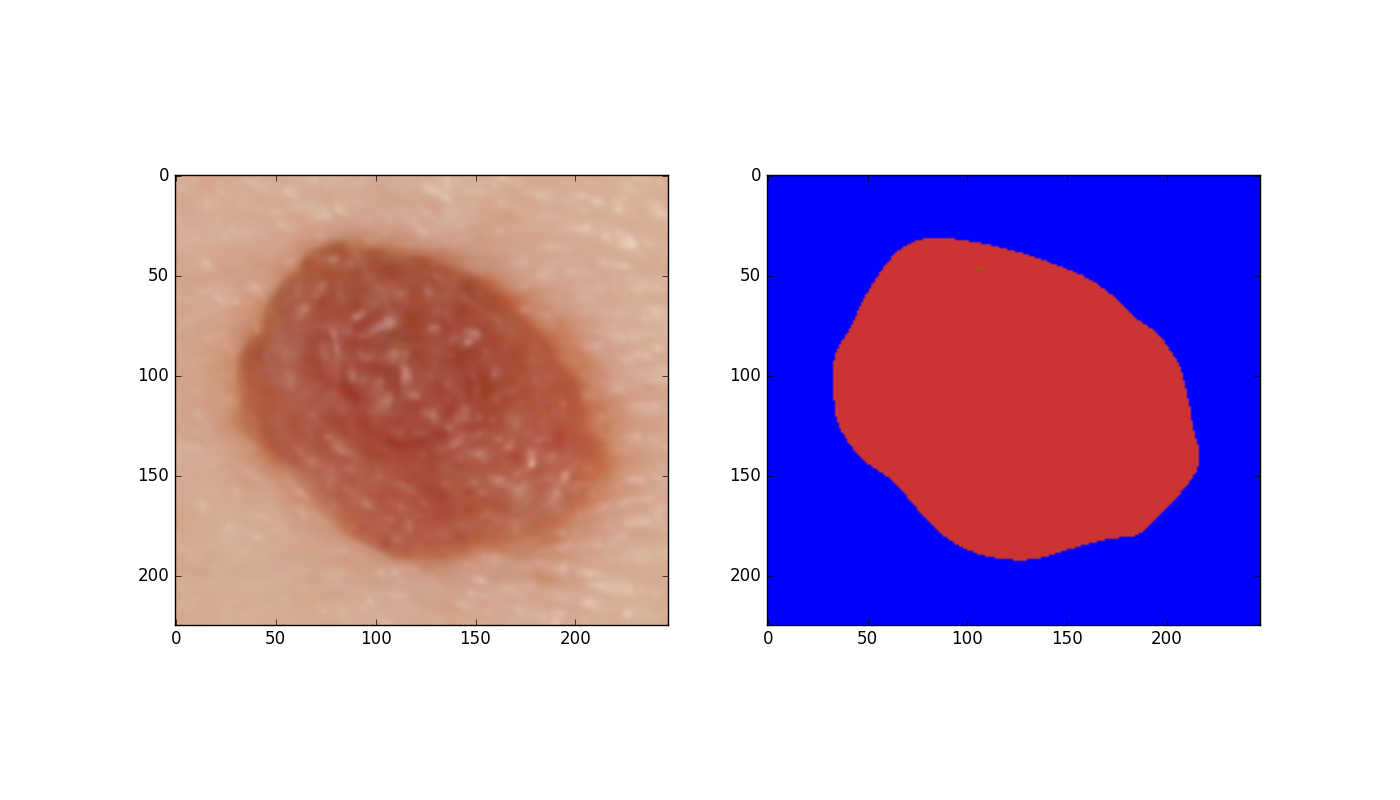
\includegraphics[height=8cm,keepaspectratio]{assets/color/examples/color_1.png}
    \caption{Example of color score 1}
    \label{fig:color_1}
\end{figure}
\begin{figure}[H]
    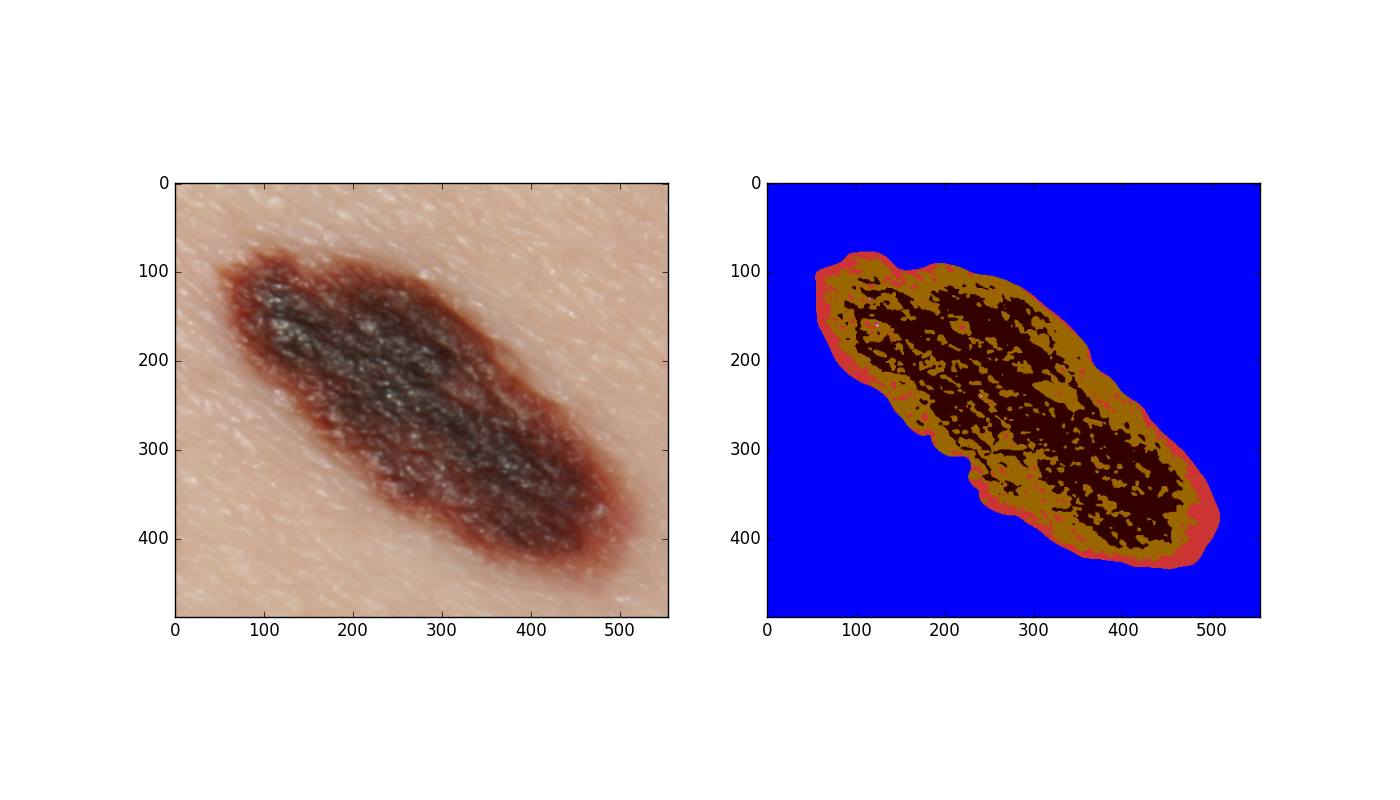
\includegraphics[height=8cm,keepaspectratio]{assets/color/examples/color_3.png}
    \caption{Example of color score 3}
    \label{fig:color_3}
\end{figure}
\begin{figure}[H]
    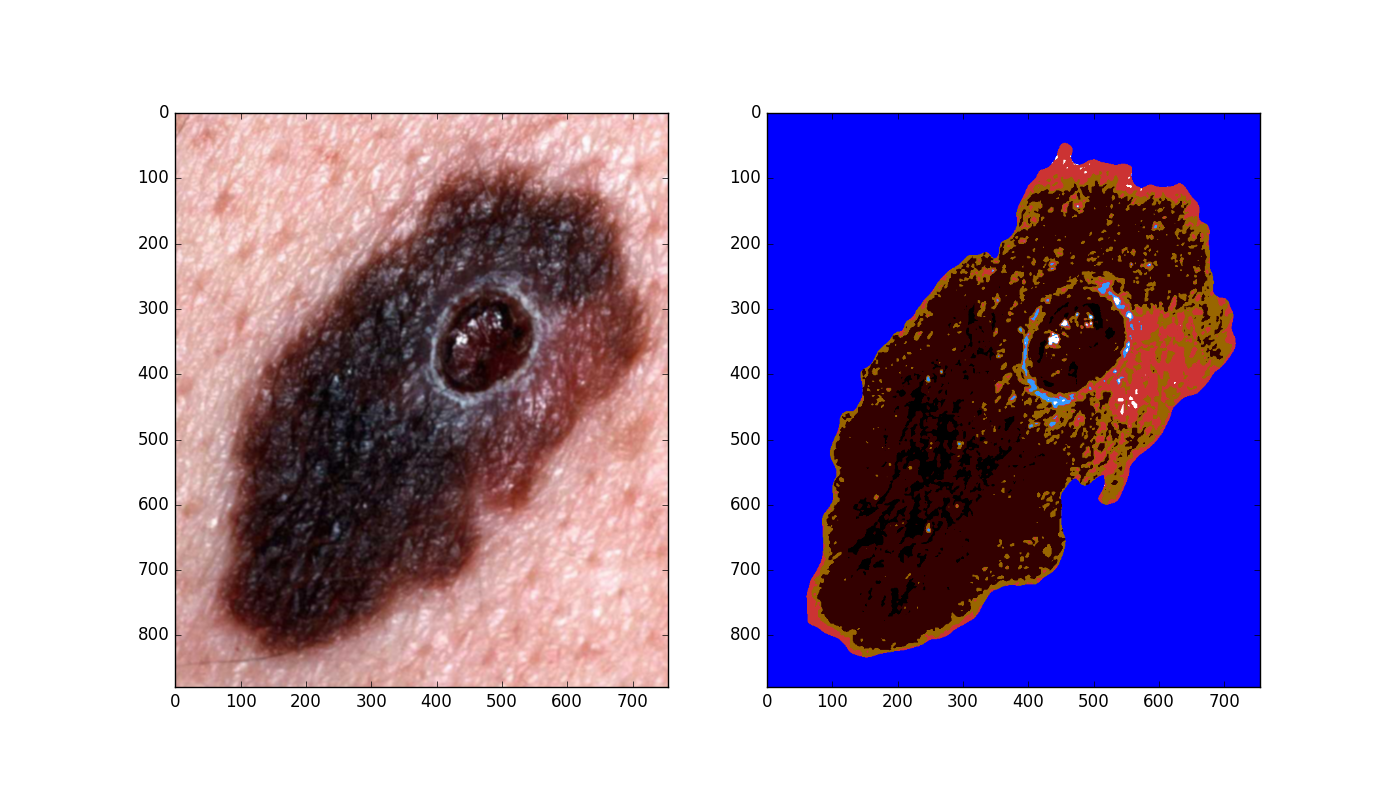
\includegraphics[height=8cm,keepaspectratio]{assets/color/examples/color_4.png}
    \caption{Example of color score 4}
    \label{fig:color_4}
\end{figure}

%\section{Two Examples}
%\subsection{Postitiv Example}

%\subsection{False Example}

%TDS Values were calculated but classification result was false.

\section{Results of Algorithm}

The results of the algorithm unfortunatale are not great. It is difficult to judge though whether this is due to the algorithm itself or the quality or the border extraction algorithm on the images provied. The PH2 image set should not be considered in the results becuse the images do not really provide an accurate reflextion of images that would be caputed by a mobile camera. The Dermquest image are a better fit for this, but the selection is much smaller.

\begin{longtable}{ | l | l | l | l | l |}
\hline
Source & False Positives & False Negatives & Correct & Total \\ \hline
Dermofit & 10 & 8 & 115 & 133 \\
Dermquest & 10 & 4 & 32 & 46 \\
PH2 & 13 & 0 & 29 & 42 \\
\hline
\caption{Results of TDS calculation}
\label{fig:tda_overview}
\end{longtable}
\begin{longtable}{ | l | l | l | l | }
\hline
Source & Malignagt & Malignant Correct & Total \\ \hline
Dermofit & 16 & 8 & 133 \\
Dermquest & 16 & 12 & 46 \\
PH2 & 0 & 0 & 42 \\
\hline
\caption{Correctly Diagnosed Malignant Melanoma Images}
\label{fig:tds_correct_mal}
\end{longtable}

